\begin{figure*}[t!]
\vspace*{-4ex}
\centering
%\setlength{\tabcolsep}{3pt} % Default value: 6pt
%\renewcommand{\arraystretch}{0.5} % Default value: 1
%
%\begin{tabular}{lll}
%
%\begin{tabular}{c} 
%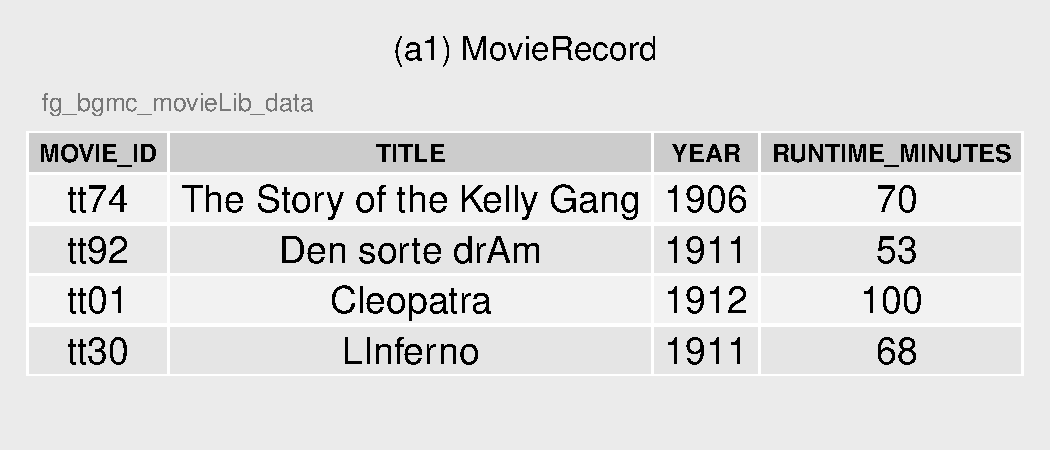
\includegraphics[width=0.33\textwidth]{../_Figures/fg_bgmc/fg_bgmc_movieLib_data_a1} \\
%\\[1ex]
%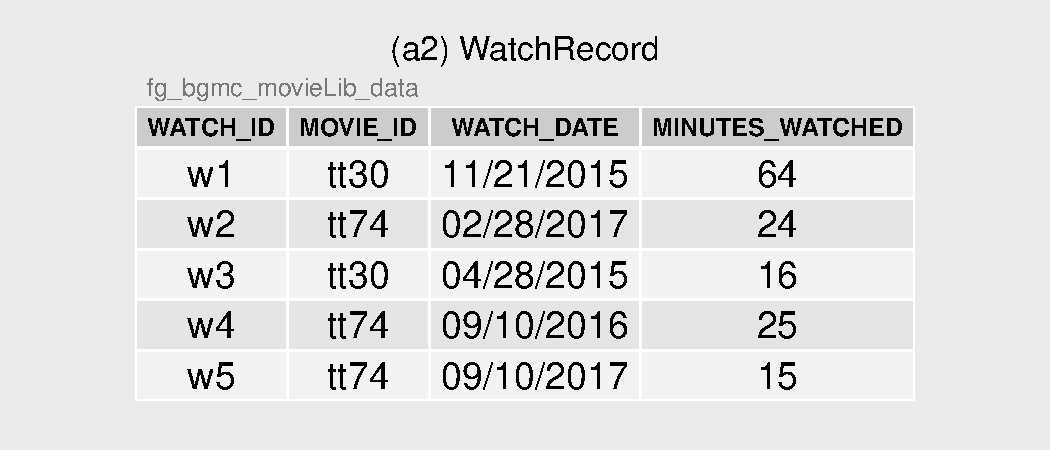
\includegraphics[width=0.33\textwidth]{../_Figures/fg_bgmc/fg_bgmc_movieLib_data_a2} \\
%\end{tabular} 
%
%&
%
%\begin{tabular}{c} 
%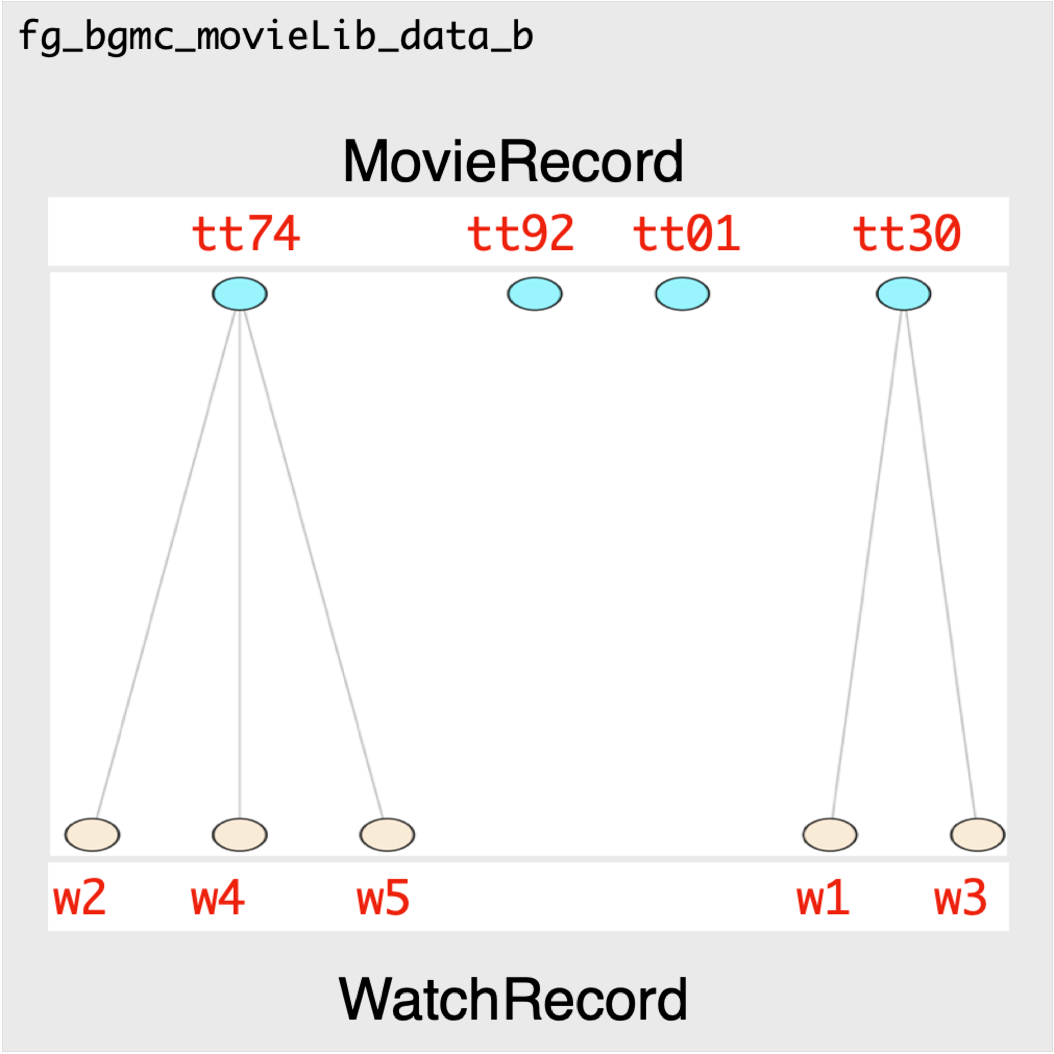
\includegraphics[width=0.31\textwidth]{../_Figures/fg_bgmc/fg_bgmc_movieLib_data_b}
%\end{tabular}
%
%&
%
%\begin{tabular}{c} 
%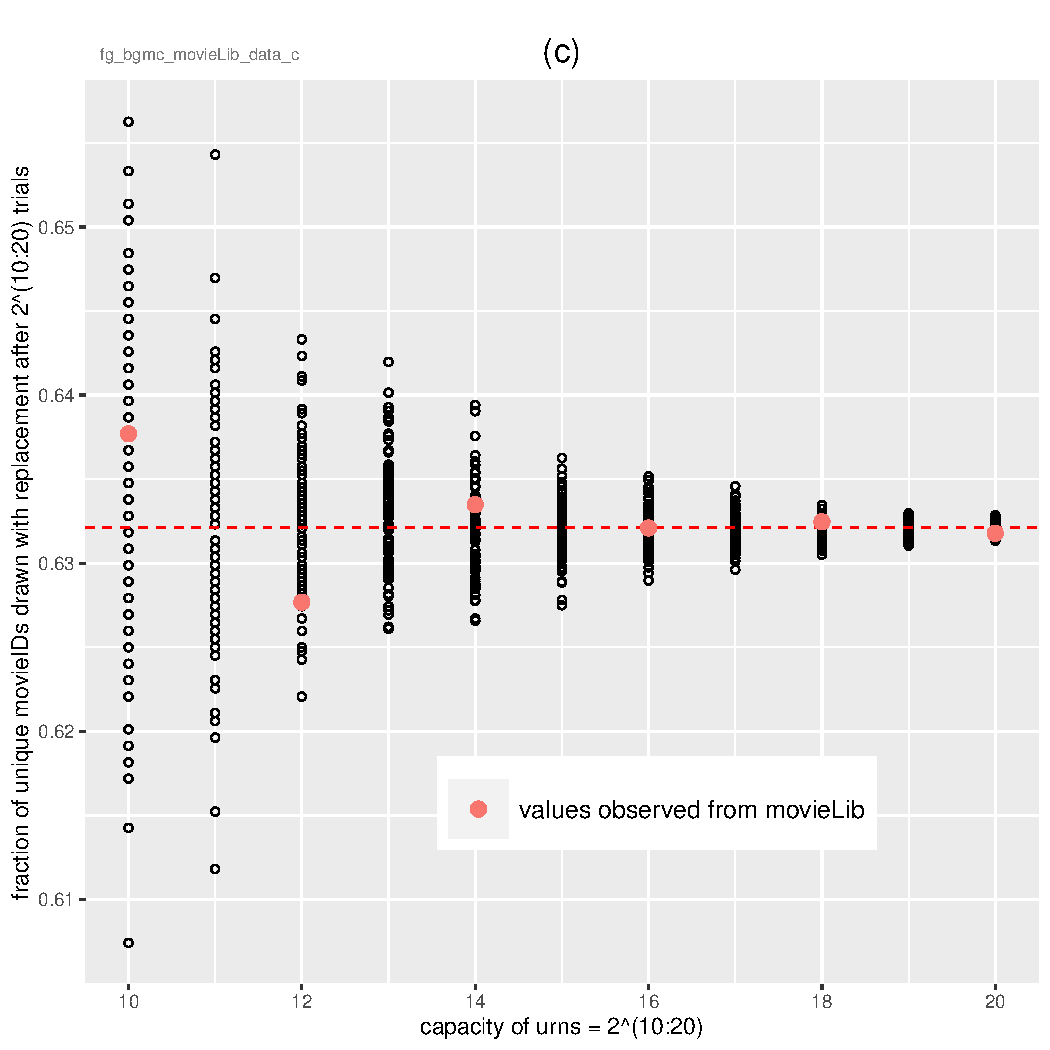
\includegraphics[width=0.33\textwidth]{../_Figures/fg_bgmc/fg_bgmc_movieLib_data_c}
%\end{tabular}
%
%\end{tabular} 

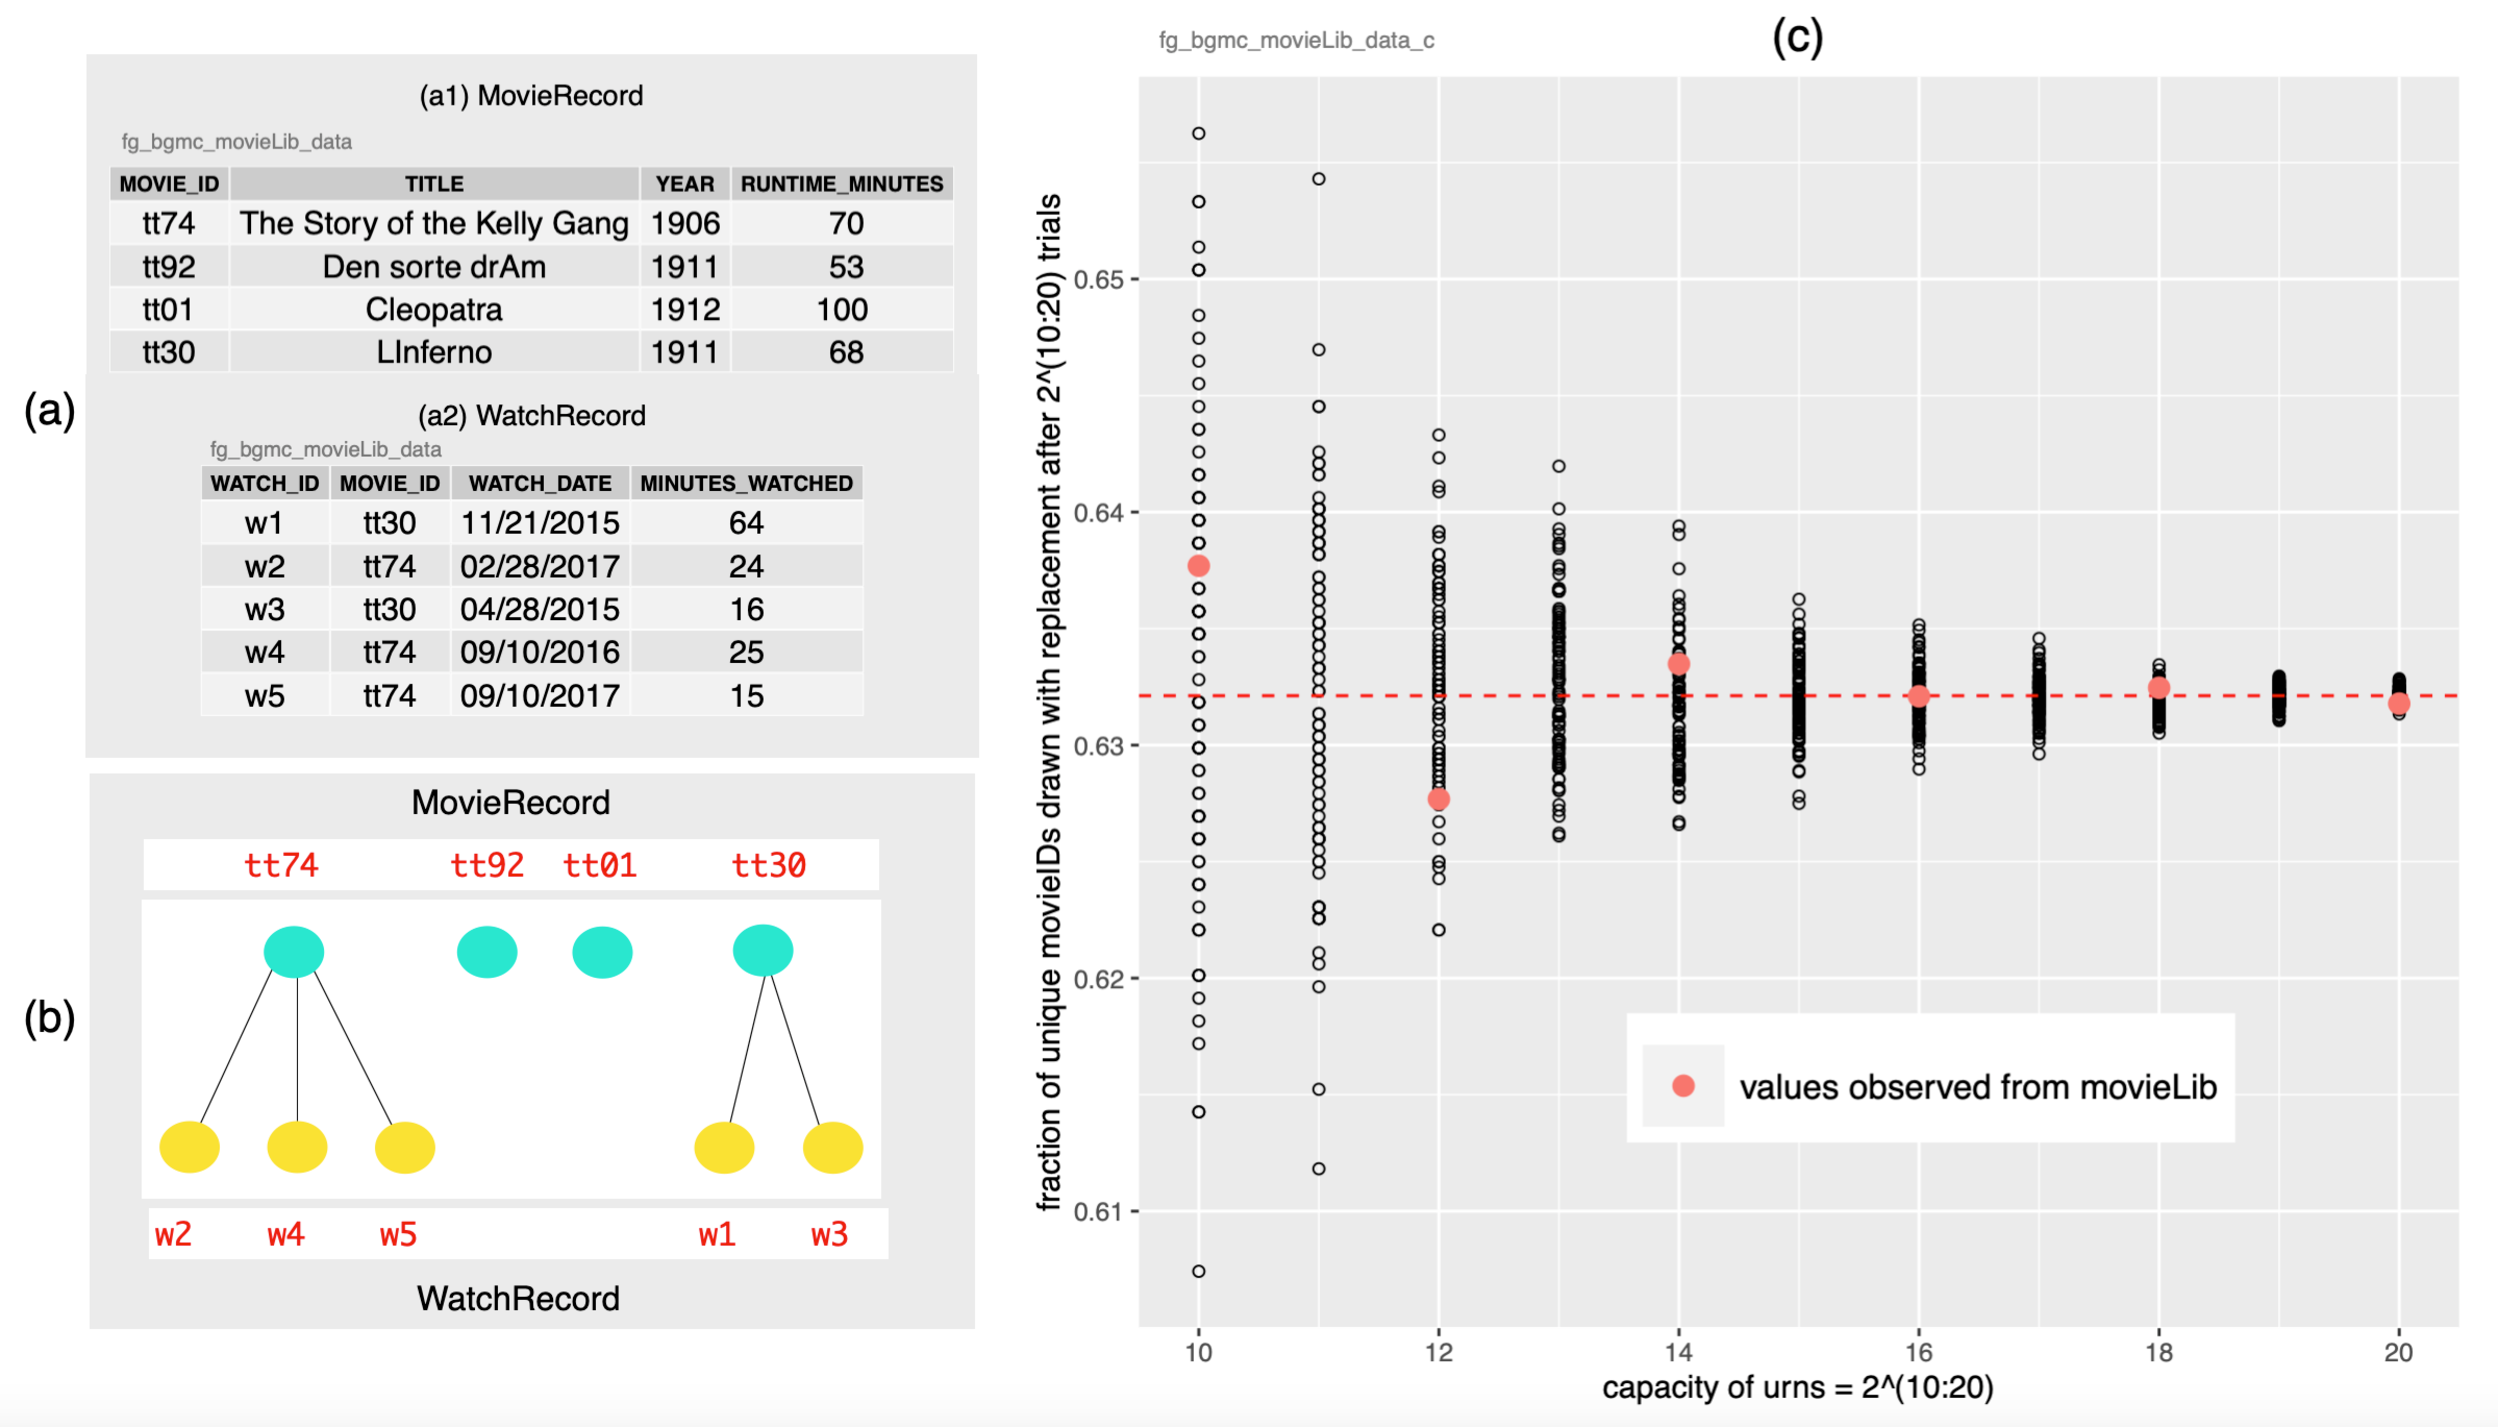
\includegraphics[width=1.00\textwidth]{_Figures/fg_bgmc_movieLib_data_abc}

\caption{Representations of data sets used in the performance experiments with 
the {\it MovieLib}   
data set introduced in Section~\ref{sec_316}:
{\sf (a)}~a tabular organization of files {\it MovieRecord} and  {\it WatchRecord}, 
{\sf (b)}~a bigraph that illustrates relationships between the
items from the two files in (a), and
{\sf (c)}~a statistical model, based on $2^{10}~...~2^{20}$ trials of sampling with replacement   
from 11 urns, each with urn capacity of holding $2^{10}~...~2^{20}$ unique  {\it movieID} tags.
The actual {\it MovieLib}  is represented with 6 urns: their sizes are
$2^{10}$,  $2^{12}$,  $2^{14}$, $2^{16}$, $2^{18}$,  and $2^{10}$.
Notably, the fraction of unique  {\it movieID} tags observed by analyzing actual data from  {\it MovieLib} 
is also converging towards $1 - e^{-1} = 0.6321$ and
is well within the expected range for this experiment.
}

%including tables with four movie information in MovieRecord and five watch histories in WatchRecord, a bipartite graph that defines the relationship between these two tables, and a plot that defines the ratio from movieLib data with size from $2^{10}$ to $2^{20}$ between the total number of movies in movie records and the number of watched movies in watch records. The red dots are the actual ratios for each dataset. }
\label{fg_bgmc_movieLib_data}
\end{figure*}
\vspace*{-4ex}